%
% A simple LaTeX template for Books
%  (c) Aleksander Morgado <aleksander@es.gnu.org>
%  Released into public domain
%
\RequirePackage{lineno}
\linenumbers 
\documentclass{article}
\usepackage[a4paper, top=3cm, bottom=3cm]{geometry}
%\usepackage[latin1]{inputenc}
%\usepackage{setspace}
\usepackage{fancyhdr}
%\usepackage{tocloft}
\usepackage{verbatim}
\usepackage{graphicx,amsmath,epsfig,color,amsfonts,relsize,subfigure}
\usepackage{authblk}
\usepackage[pdftex]{graphicx}
\usepackage{sidecap}
%\usepackage[running]{lineno}
\newcommand{\fbinv} {\mbox{\ensuremath{\,\text{fb}^\text{$-$1}}}}
\begin{document}

 
%\pagestyle{empty}
%\begin{flushleft}
\pagenumbering{}
% Set book title
\title{\textbf{Long Baseline Neutrino Facility}}

\author{Ekaterina Avdeeva}

\affil{University of Nebraska-Lincoln, USA}
\maketitle
%\end{flushleft}

\begin{abstract}
The paper reviews the techniques of the Long Baseline Neutrino Facility, which is currently under construction, as the most ambitious experiment to study neutrino oscillations in the World. General properties of neutrinos, theoretical and historical backgrounds of the oscillations, techniques and achievements of several other experiments are also discussed. The paper is prepared as a part of the author's Comprehensive Exam at the Physics\&Astronomy Department of the University of Nebraska-Lincoln.
\end{abstract}

% 2nd page, thanks message
%-------------------------------------------------------------------------------
%\thispagestyle{empty}
%\newpage


% General definitions for all Chapters
%-------------------------------------------------------------------------------

% Define Page style for all chapters
\pagestyle{fancy}
% Delete the current section for header and footer
\fancyhf{}
% Set custom header
\lhead[]{\thepage}
\rhead[\thepage]{}

% Set arabic (1,2,3...) page numbering
\pagenumbering{arabic}
\tableofcontents

%
% Not enumerated chapter
%-------------------------------------------------------------------------------
%\linenumbers

\clearpage
\section{Introduction. Neutrinos as Fundamental Standard Model Particles}

The Standard Model can be summarized in a table like one at fig. \ref{fig:StandardModel}. It includes three charged leptons, three neutrinos and six quarks and their antiparticles which are splitted into three generations. In addition, it includes gauge bosons, Higgs boson and three fundamental interactions: electromagnetic, strong and weak. Charged particles, which include three leptons (electrons, muons and $\tau$-leptons), all quarks, W-bosons and their antiparticles can interact electromagnetically, through exchange of virtual photon. Quarks also posses additional quantum number which is called "color" and can also participate in strong couplings, through exchange of gluons. All those particles and also neutrinos can interact through weak interactions through charged current (CC), by exchanging W-boson, and through neutral current (NC), by exchanging Z-boson. The corresponding Feynmann diagrams for the NC and CC are shown at fig. \ref{fig:NuScattering}\\

\begin{figure}
\caption{Fundamental particles and interactions. Three generations of fundamental particles and interaction mediators. Charged leptons and quarks are subjects to electromagnetic interactions (through photons). Quarks can also interact strongly (through gluons). All leptons and quarks can interact weakly (through $W^{\pm}$ and $Z^0$ bosons). All these and only these fundamental particles are discovered at the moment. Source of picture: \cite{ref_fig_StandardModel}}
\label{fig:StandardModel}
\centering 
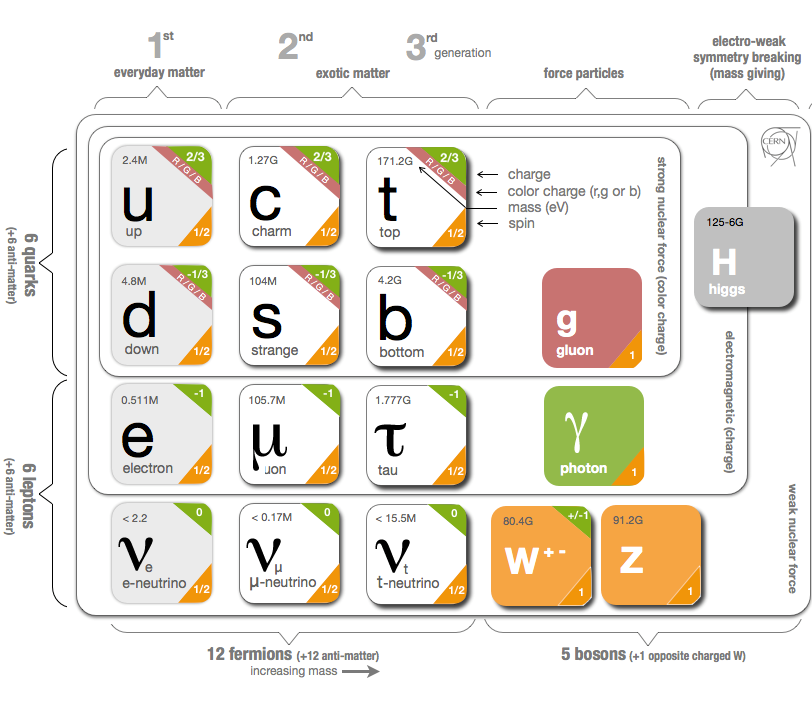
\includegraphics[width=0.83\textwidth, keepaspectratio=true]{figs/StandardModel.png}
\end{figure}

\begin{figure}
\caption{Feynmann diagrams of neutral current (NC, left), and neutral current (CC, middle and right) neutrino scattering.}
\label{fig:NuScattering}
\centering
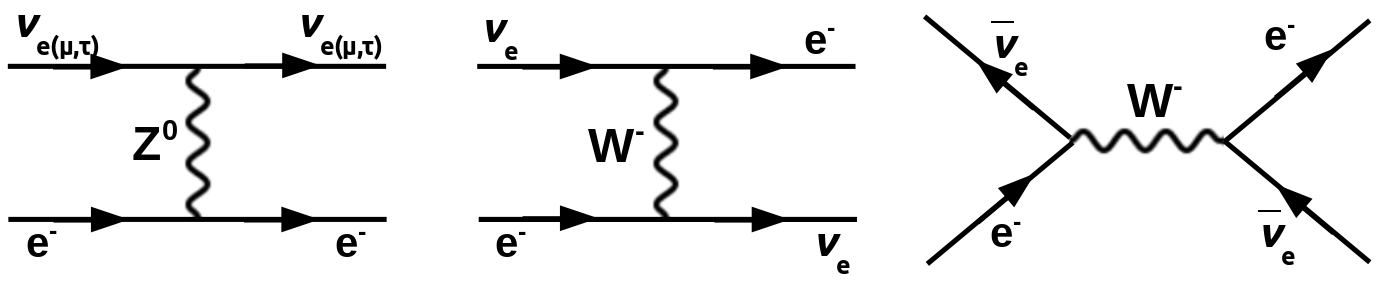
\includegraphics[width=0.98\textwidth, keepaspectratio=true]{figs/neutrinoScattering.png}
\end{figure}


All known substance in the Universe consists of millions of different molecules which are composed by hundreds different atoms. Each atom consists of certain number of protons, neutrons and electrons. All protons and neutrons are composed of three quarks (uud for proton and udd for neutron) which are glued together by strong interactions. Therefore, all known substance consists on only three fundamental particles from the fig. \ref{fig:StandardModel}: u- and d-quarks and electrons. Despite neutrinos are not part of substances, large number of them exist in the nature, without any human-built machines. Quoting \cite{ref_Griffiths}, 11.1: "John Bahcall, who was responsible for most of the calculations of solar neutrino abundances, liked to say that 100 billion neutrinos pass through your thumbnail every second; and yet they are so ethereal that you can look forward to only one or two neutrino-induced reaction in your body during your entire lifetime".\\
Two very common and well known interactions with neutrino participation are neutron beta decay and muon decay. The Feynmann diagrams of these processes are shown at fig. \ref{fig:MuonAndNeutronDecays}. Mean lifetime of free neutron is $~15$ minutes and $>99.9\%$ of those which decay will do it though the beta decay: $n \rightarrow p + e^- + \bar{{\nu}_e} $ \cite{ref_PDG}. At the level of fundamental particles, neutron consists of two d-quarks and one u-quark and in the beta decay one of the d-quarks transfers to u-quark though the weak interaction mediated by $W^- $ boson. Thus, the proton, which consists of two u-quarks and one d-quark, is being produced. When this happens, the electron and electron antineutrino are emitted to preserve the charge and the lepton flavor number conserved. The examples of the neutron beta decay in nature include ${^{49}}{_{19}}K \rightarrow {^{40}}{_{20}}Ca$, ${^{64}}{_{29}}Cu \rightarrow {^{64}}{_{30}}Zn$, ${^3}{_1}H \rightarrow {^3}{_2}He$ \cite{ref_Griffiths} (the positive beta decay,  $p \rightarrow n + e^+ + {\nu}_e $, is not possible for free proton but it can happen when a proton is part of a nuclei). As for a muon, it's mean lifetime is $~2 {\mu}s$ and $~99\%$ of muons which decay would do that to electron, muon neutrino and electron antineutrino as ${\mu}^- \rightarrow e^- + {\nu}_{\mu} + \bar{{\nu}_e}$ through the W boson. This process is also common in nature, in cosmic rays: muons are produced in the upper layers of the Earth atmosphere from the interaction of the particles coming from cosmics with the atmosphere molecules, for instance, as $p+p \rightarrow n+p+\pi^+$ with further pion decay $\pi^+ \rightarrow \mu^+ + \nu_\mu$ and then some number of muons decay $\mu^+ \rightarrow e^+ + \nu_e + \bar{\nu_\mu}$ while traveling through the atmosphere to the ground. The scheme of the shower in the Earth atmosphere induced by the primary incident proton is shown on fig. \ref{fig:cosmicMuons}.   

\begin{figure}
\caption{Feynmann diagrams of (left) neutron and (right) muon decays. Neutron beta decay \cite{ref_fig_NeutronDecay}(d-quark of transfers to u-quark through the W-boson with emission of electron and antineutrino). Muon decay \cite{ref_fig_MuonDecay}(muon decays to electron, neutrino and antineutrino through W-boson}
\label{fig:MuonAndNeutronDecays}
\centering
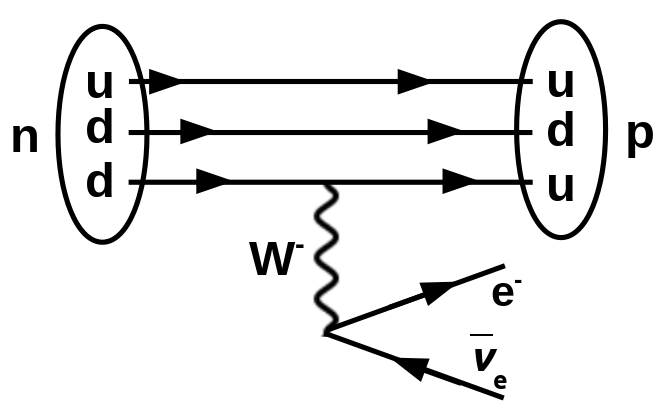
\includegraphics[width=0.35\textwidth, keepaspectratio=true]{figs/NeutronBetaDecay.png}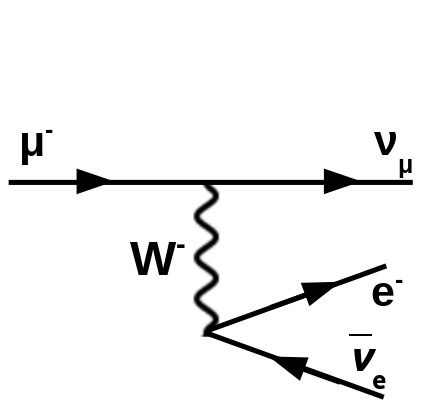
\includegraphics[width=0.35\textwidth, keepaspectratio=true]{figs/MuonDecay.png}
\end{figure}

\begin{SCfigure}
\caption{Cosmic shower induced by scattering of the incident cosmics proton of an air molecule. Charged and neutron pions are born in the reaction and then they further decay as $\pi^0 \rightarrow \gamma\gamma$, $\pi^+ \rightarrow \mu^+ + \nu_\mu$, $\pi^- \rightarrow \mu^- + \bar{\nu_\mu}$.}
\label{fig:cosmicMuons}
\centering
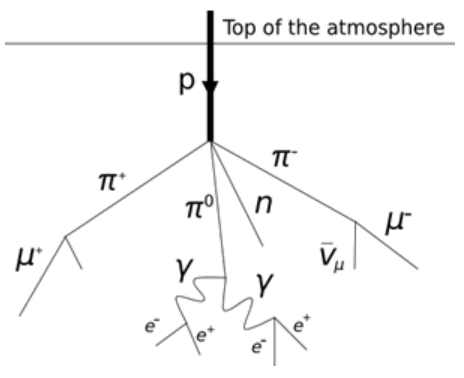
\includegraphics[width=0.60\textwidth, keepaspectratio=true]{figs/cosmicMuons.png}
\end{SCfigure}



There are three flavors of neutrino, one for each generation: electron neutrino, muon neutrino, $\tau$-neutrino. And in the processes described above (neutron beta decay and muon decay) the lepton flavor numbers $L_e$, $L_{\mu}$ and $L_{\tau}$ are conserved. The table \ref{tab:LeptonFlavorNumber} shows the value of this number for all leptons and antileptons. 

\begin{table}[h]
  \begin{center}
  \caption{ Lepton Flavor Number}
  \begin{tabular}{|c|c|c|c|}
     particles & $L_e$ & $L_{\mu}$ & $L_{\tau}$ \\ \hline
     $e^-,\nu_e$ &  +1  &  0  &  0  \\ \hline 
     $e^+, \bar{\nu_e}$ &  -1  &  0  &  0  \\ \hline 
     $\mu^-,\nu_{\mu}$ &  0  &  +1  &  0  \\ \hline 
     $\mu^+, \bar{\nu_{\mu}}$ &  0  &  -1  &  0  \\ \hline 
     $\tau^-,\nu_{\tau}$ &  0  &  0  &  +1  \\ \hline 
     $\tau^+, \bar{\nu_{\tau}}$ &  0  &  0  &  -1  \\ \hline 
  \end{tabular}
  \label{tab:LeptonFlavorNumber}
  \end{center}
\end{table}

The lepton flavor numbers are conserved in almost all particle physics processes and the only violation of this law observed by this time is the neutrino oscillations - the ability of neutrino to change flavor. 

This paper reviews the theoretical background and the most important experimental measurements related to the neutrino oscillations, related open physics questions which raised over the last several decades, and techniques of the future experiment Long Baseline Neutrino Facility and the anvantages it will have over the other experiments of this kind.  


\clearpage
\section{Neutrino Oscillations. Theory}

\subsection{Model of Two-Neutrino Oscillations in Vacuum}
Lets consider two neutrinos case as it's described in the chapter 11 of the Griffiths textbook \cite{ref_Griffiths}.\\
Suppose there are only two neutrinos $\nu_e$ and $\nu_{\mu}$. Then true stationary states of the system would be the orthogonal combinations:\\

\begin{center}
$\nu_1=\nu_{\mu}cos\theta-\nu_esin\theta$\\
$\nu_2=\nu_{\mu}sin\theta+\nu_ecos\theta$\\
\end{center}

Then, according to the quantum mechanics,\\
\begin{center}
$\nu_1(t)=\nu_1(0)e^{\frac{-iE_1t}{\hbar}}$, $\nu_2(t)=\nu_2(0)e^{\frac{-iE_2t}{\hbar}}$\\
\end{center}

Suppose, at t=0 there were $\nu_e(0)=1$, $\nu_\mu(0)=0$\\
Then 
\begin{center}
$\nu_1(0)=-sin\theta$, $\nu_2(0)=cos\theta$, $\nu_1(t)=-{sin\theta}e^{\frac{-iE_1t}{\hbar}}$, $\nu_2(t)=-{cos\theta}e^{\frac{-iE_2t}{\hbar}}$\\
\end{center}

Thus, we are getting the system:\\
\begin{center}
$-{sin\theta}e^{-{{iE_1t} \over \hbar}}=\nu_\mu(t)cos\theta-\nu_e(t)sin\theta$,\\
$-{sin\theta}e^{-{{iE_2t} \over \hbar}}=\nu_\mu(t)sin\theta-\nu_e(t)cos\theta$\\
\end{center}

By solving this sytem for $\nu_e$ and $\nu_\mu$, one would get\\
\begin{center}
$P_{\nu_e \rightarrow \nu_\mu}=|\nu_\mu(t)|^2=[{sin2\theta}sin{\frac{(E_1-E_2)t}{2\hbar}}]^2$,\\
$P_{\nu_e \rightarrow \nu_e}=|\nu_e(t)|^2=1-[{sin2\theta}sin{\frac{(E_1-E_2)t}{2\hbar}}]^2$\\
\end{center}

Thus, for freely travelling neutrinos, if $\nu_e$ was emmitted, at any point there is a certain probability to register $\nu_e$ or $\nu_\mu$ and those probablities change with time periodically, by $~[sin(At)]^2$ law. That's why the phenomenon is called the neutrino oscillations.
Suppose momenta $p_1=p_2$. Then using $E^2=p^2+m^2$ and assuming $m_{1,2}<<E_{1,2}$, the probablities will take forms of\\
\begin{center}
$P_{\nu_e \rightarrow \nu_\mu}=|\nu_\mu(t)|^2=[{sin2\theta}sin{\frac{(E_1-E_2)t}{2\hbar}}]^2=[{sin2\theta}sin{\frac{(m_1^2-m_2^2)c^3}{4\hbar{E}}z}]^2$\\  
\end{center}

\subsection{Mechanism of Neutrinos Getting Mass}

\subsection{Three-Neutrino Oscillation}

Three neutrino case is described in the "Long-baseline Neutrino Oscillation Physics" section of the draft Conteptual Design Report (CDR) of the Long Baseline Neutrino Facility (LBNF). For three neutrino case, the oscillations are determined by complex unitary matrix which is called Pontecorvo-Maki-Nakagava-Sakata (PMNS) matrix:\\
\begin{center}
$ \begin{pmatrix} \nu_{e} \\ \nu_{\mu} \\ \nu_{\tau} \\ \end{pmatrix}
 = U_{PMNS}\cdot \begin{pmatrix} \nu_{1} \\ \nu_{2} \\ \nu_{3} \\ \end{pmatrix} = 
 \begin{pmatrix}
  U_{e1} & U_{e2} & U_{e3} \\
  U_{\mu1} & U_{\mu2} & U_{\mu3} \\
  U_{\tau1} & U_{\tau2} & U_{\tau3} \\
 \end{pmatrix}
 \cdot
\begin{pmatrix} \nu_{1} \\ \nu_{2} \\ \nu_{3} \\ \end{pmatrix}$\\
\end{center}
The $U_{PMNS}$ matrix depends on three neutrino mixing angles ($\theta_{12}$, $\theta_{23}$, $\theta_{13}$) and CP-violating phase $\delta_{CP}$. If define $c_{ab}=cos\theta_(ab)$, $s_{ab}=sin\theta_(ab)$, the $U_{PMNS}$ matrix can be splitted into three multipliers, each would be responsible for mixing of one pair of neutrino flavors:\\
\begin{center}
$U_{PMNS} =
 \begin{pmatrix}
  1 & 0 & 0 \\
  0 & c_{23} & s_{23} \\
  0 & -s_{23} & c_{23} \\
 \end{pmatrix}
 \cdot
 \begin{pmatrix}
  c_{13} & 0 & e^{i\delta_{CP}}s_{13} \\
  0 & 1 & 0 \\
  -e^{i\delta_{CP}}s_{13} & 0 & c_{13} \\
 \end{pmatrix}
 \cdot
 \begin{pmatrix}
  c_{12} & s_{12} & 0 \\
  -s_{12} & c_{12} & 0 \\
  0 & 0 & 1 \\
 \end{pmatrix}$ \\
\end{center}
The probability amplitudes of neutrino mixing are defined by parameters of the $U_{PMNS}$ but, analogous to simplified two-neutrino case described above, the differences of squares of neutrino masses also contribute to the probability. There are two independent expressionce for squares of masses differences: ${\Delta}m_{12}^2 = m_1^2-m_2^2$ and ${\Delta}m_{32}^2 = m_3^2-m_2^2$. Mass differences were measured in other neutrino oscillation experiments but the ${\Delta}m_{12}^2$ and ${\Delta}m_{32}^2$ present in the equations evenly and therefore the signs of these expressions were not measured. If the masses order as $m_3 > m_2 > m_1$, it's called normal neutrino mass hierarchy because other fundamental particles orders in a way that later generation particles have higher masses than lower generation particles. If the masses order as $m_1 > m_2 > m_3$ it's called inverted neutrino mass hierarchy. The mixing angles $\theta_{12}$, $\theta_{23}$, $\theta_{13}$ and differences of squared masses $|{\Delta}m_{12}^2|$ and $|{\Delta}m_{32}^2|$ are measured and give $U_{PMNS}$ matrix form of\\
\begin{center}
$|U_{PMNS}| \sim
 \begin{pmatrix}
  0.8 & 0.5 & 0.2 \\ 0.5 & 0.6 & 0.6 \\ 0.2 & 0.6 & 0.8 \\
 \end{pmatrix}$\\
\end{center}
The CP-violating phase $\delta_{CP}$ is unknown.\\*
The analogous matrix for quark mixing, Cabibbo-Kobayashi-Maskawa (CKM) matrix $V_{CKM}$, is much more diagonal:\\*
\begin{center}
$|V_{CKM}| \sim
 \begin{pmatrix}
  1 & 0.2 & 0.004 \\ 0.2 & 1 & 0.04 \\ 0.008 & 0.04 & 1 \\
 \end{pmatrix}$\\
\end{center}
One of the important questions in modern particle physics is why the quark mixing angles are so much smaller than neutrino mixing angles and the other important question is whether there is any relationship between quark and neutrino mixing matrices.\\

The \cite{ref_LBNFdoc_volume-physics} gives the following expression for $\nu_\mu \rightarrow \nu_e$ probability in presence of the Earth matter assuming it has constant density: \\
\begin{center}

\begin{equation}
\label{eq:P_bigFormula}
P(\nu_\mu \rightarrow \nu_e) \simeq P_1 + P_2 + P_3 
\end{equation}

\begin{equation}
\label{eq:P_bigFormula_1}
P_1 = sin^2{\theta_{23}}sin^2{2\theta_{13}}\frac{sin^2(\Delta_{13}-aL)}{(\Delta_{13}-aL)^2}\Delta^2_{31}
\end{equation}

\begin{equation}
\label{eq:P_bigFormula_2}
P_2 = sin2\theta_{23}sin2\theta_{13}sin2\theta_{12}\frac{sin(\Delta_{31}-aL)}{(\Delta_{31}-aL)}\Delta_{31}\frac{sin(aL)}{aL}\Delta_{21}cos(\Delta_{31}+\delta_{CP})
\end{equation}

\begin{equation}
\label{eq:P_bigFormula_3}
P_3 = cos^2\theta_{23}sin^2{2\theta_{12}}\frac{sin^2(aL)}{(aL)^2}\Delta^2_{21}
\end{equation}

where $\Delta_{ij}={\Delta}m^2_{ij}L/4E$, and $a={G_F}{N_e}/sqrt(2)$\\
\end{center}

For $P(\bar{\nu_\mu} \rightarrow \bar{\nu_e})$ one would need to change $\delta_{CP} \rightarrow -\delta_{CP}$ (bacuuse of neutrino-antineutrino assymetry for CP-violationg phase) and $a \rightarrow -a$ (because only electrons present in the Earth, not positrons). The effect of $a \rightarrow -a$ increases with L which means more sensitivity to mass hierarchy for experiments with larger baseline. The planned baseline of the LBNF is 1300 km and it's expected to be enough to determine the neutrino mass hierarchy and also the CP-violation phase.

\begin{figure}
\caption{$P(\nu_\mu \rightarrow \nu_e)$ at a baseline of 1300 km}
\label{fig:LBNF_oscProbability}
\centering
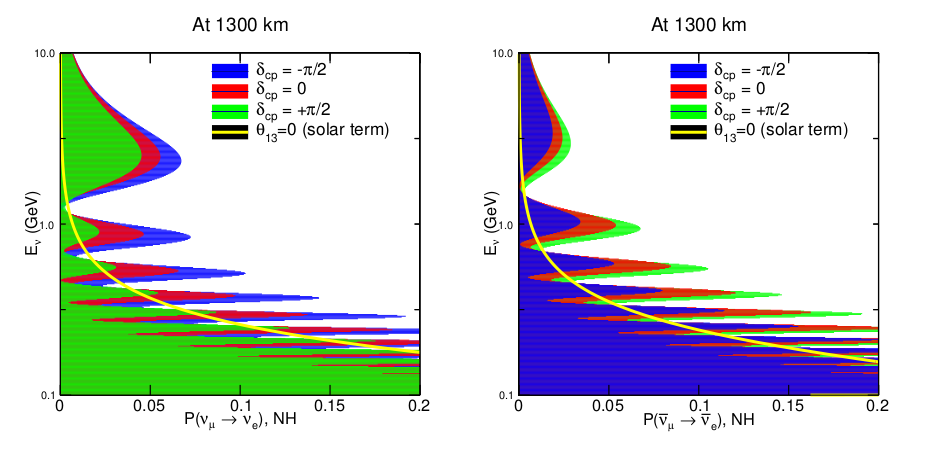
\includegraphics[width=0.98\textwidth, keepaspectratio=true]{figs/LBNF_oscProbability.png}
\\$P(\nu_\mu \rightarrow \nu_e)$ at a baseline of 1300 km, as a function of neutrino energy. Left - neutrinos, right - antineutrinos. Figure is taken from the LBNF CDR draft, volume physics\cite{ref_LBNFdoc_volume-physics}
\end{figure}

The figure \ref{fig:LBNF_oscProbability} shows that magnitude and frequency of oscillations both depend on $\delta_{CP}$ and the differences become more significant for higher oscillation nodes which correspond to lower energies of neutrino/antineutrino. Since changes due to different $\delta_{CP}$s are opposite for neutrinos and antineutrinos, it's important for the experiment to operate both.\\


\clearpage
\section{Neutrino Oscillations. History and Status}
%\subsection{First Discovery and Confirmation}

The history of the discovery of neutrino oscillations is described in \cite{ref_Griffiths}, chapter 11. The first evidence of neutrino oscillations was seen in the Homestake experiment in 1968 with solar neutrinos. This experiment used a Chlorino radiochemical detector. Neutrinos interacted with chlorine-37 atoms and converted them to argon-37 through the reaction $\nu_e+^{37}Cl \rightarrow ^{37}Ar+e$ or, at the more fundamental level, $\nu_e+n \rightarrow p+e$. The argon atoms were then separated and counted. The experiment registered a number of neutrinos three times smaller than theoretically predicted. The phenomenon was called the ``solar neutrino problem".  The detector was sensitive to electron neutrinos only. Soon after Bruno Pontecorvo proposed the explanation to the solar neutrino problem that neutrino can change its flavor on its way from the Sun to the detector. The theory was confirmed  by Super-Kamiokande and Sudbury Neutrino Observatory (SNO) collaborations. \\ \\
The Super-Kamiokande experiment used a water detector and could register any sort of neutrino through $e+\nu \rightarrow e+\nu$ scattering. However the NC scattering can not distinguish between different neutrino flavors. Also, electron neutrinos could interact through CC, which made the detection efficiency of electron neutrinos 6.5 times higher than other flavors (the left Feynman diagram in Fig. \ref{fig:NuScattering} is possible for any neutrino flavor but the middle and right diagrams are possible only for electron neutrino). Therefore, Super-Kamiokande was able to register any neutrino but could not distinguish between neutrino flavor and had lower detection efficiency for non-electron neutrinos. They assumed all neutrinos to be electron neutrinos and recorded $45\%$ of the predicted amount. Then the SNO, which used heavy water and was able to distinguish the electron neutrino flux from the total neutrino flux, confirmed that some of the neutrinos coming from the Sun are detected as $\nu_\mu$ or $\nu_\tau$. The reactions in the working volumes of the three detectors can be summarized as the following:\\ 
\begin{itemize}
\item Homestake experiment (1968): $\nu_e + ^{37}Cl \rightarrow ^{37}Ar+e$
\item Super-Kamiokande experiment (1998): $\nu + e \rightarrow \nu + e$ 
\item Solar neutrino observatory (2002): $\nu_e + d \rightarrow p+p+e$, $\nu+d \rightarrow n+p+\nu$, $\nu+e \rightarrow \nu+e$
\end{itemize}
The SNO reported $\nu_e$ flux to be $35\%$ of the predicted flux. Comparing it to the Super-Kamiokande results and knowing that Super-Kamiokande was 6.5 times less sensitive to $\nu_\mu$ and $\nu_\tau$, one obtains:\\ \\
$N_{SNO}=0.35 \cdot N_{th}$,\\ \\
$N_{SK}^{CORR1}=0.45 \cdot N_{th}=0.35 \cdot N_{th}+0.1 \cdot N_{th}$,\\ \\
$N_{SK}^{CORR1}=\frac{N_{SK}^{REG}}{\epsilon^{e}}=0.45 \cdot N_{th} $,\\ \\
$N_{SK}^{CORR2}=\alpha \cdot \frac{N_{SK}^{REG}}{\epsilon^{e}}+(1-\alpha) \cdot \frac{N_{SK}^{REG}}{\epsilon^{\mu/\tau}}=\alpha \cdot \frac{N_{SK}^{REG}}{\epsilon^{e}}+(1-\alpha) \cdot \frac{N_{SK}^{REG}}{\epsilon^{e}/6.5}$,\\ \\
$\alpha=0.35/0.45$,\\ \\
$N_{SK}^{CORR2}=0.35 \cdot N_{th}+0.65 \cdot N_{th}=N_{th}$,\\ \\
where $N_{th}$ is a number of theoretically predicted neutrinos, $N_{SNO}$ is a number of neutrinos registered by the SNO experiment corrected by the neutrino detection efficiency, $N_{SK}^{REG}$ is a number of neutrinos registered by Super-Kamiokande, $N_{SK}^{CORR1}$ is a number of neutrinos registered by Super-Kamiokande corrected by the electron detection efficiency, $\epsilon^{e}$ is the electron detection efficiency, $N_{SK}^{CORR2}$ is a number of neutrinos registered by Super-Kamiokande corrected in assumption that part of registered neutrinos were $\nu_e$ and the other part were $\nu_\mu$ or $\nu_\tau$. This result confirmed the neutrino socillations theory and resolved the solar neutrino problem.\\ \\
%\subsection{First measurements of the neutrino oscillation parameters}
There are four types of experiments which allow to study neutrino properties: solar, atmospheric, reactor, and accelerator neutrino experiments \cite{ref_PDG}. The idea of any neutrino oscillation measurement is to observe and quantify disappearance of $\nu_f$($\bar{\nu_f}$) and/or appearance of $\nu_{f'}$($\bar{\nu_{f'}}$), where f is a flavor of neutrinos produced in the reaction in the Sun, atmosphere, reactor or target, and $f'$ is the flavor of neutrinos which were not produced in the reaction.\\ \\
The Sun is a source of electron neutrinos. They are produced in the reaction $4p \rightarrow {^4}He+2e^{+}+2\nu_{e}$. Solar neutrino experiments (as the three described above) focus on the disappearance of $\nu_e$ and appearance of $\nu_\mu$ or $\nu_\tau$. These experiments are characterized by very long baselines (distance from the Sun to the Earth, $\simeq 1.5 \cdot 10^8$ km) and neutrino energies of $\sim 1$ MeV. Solar neutrino experiments are sensitive to ${\Delta}m^2_{21}={\Delta}m^2_{Sol}$, which is also called Solar mass splitting. Matter effects in the Sun makes such experiments sensitive to the sign of ${\Delta}m^2_{21}$, and it was determined that $m2>m1$ \cite{ref_presentation_NH}. The Solar neutrino experiments also provided the first measurements of the mixing angle $\theta_{12}$.\\ \\
The nuclear reactors produce $\bar{\nu_e}$s in beta decay of radioactive elements as $n \rightarrow p + e^- + \bar{\nu_e}$, and then antineutrinos further oscillate and are detected. Typical baselines of such experiments vary from 1 to 100 km, and the energies of emitted antineutrinos are $\sim 1$ MeV. Reactor experiments provide measurements of ${\Delta}m^2_{21}$, $\theta_{12}$, and $\theta_{13}$.\\ \\
The source of atmospheric neutrinos is cosmic rays scattering from air molecules as shown in Fig. \ref{fig:cosmicMuons}. Pions produced in the air decay as $\pi^{\pm} \rightarrow \mu^{\pm}+\nu_\mu(\bar{\nu_\mu})$ with further muon decay as $\mu^{\pm} \rightarrow e^{\pm}+\nu_e(\bar{\nu_e})+\bar{\nu_\mu}(\nu_\mu)$, which lead to a flux ratio $\Phi(\nu_\mu+\bar{\nu_\mu}):\Phi(\nu_e+\bar{\nu_e}) \approx 2:1$. Baselines of atmospheric neutrinos experiments are $\sim 10^4$ km, and neutrino energies are $\sim 1$ GeV. Atmospheric neutrino experiments are more sensitive to ${\Delta}m^2_{32}={\Delta}m^2_{Atm}$, which is also called atmospheric mass splitting, and also provide measurements of $\theta_{23}$. Such experiments are also potentially capable of measuring CP-violating phase $\delta$, but experiments has been performed so far were not sensitive enough to measure $\delta$. \\ \\
Accelerators can produce $\nu_\mu$ or $\bar{\nu_\mu}$ similarly as $\nu_\mu$/$\bar{\nu_\mu}$ are produced in the atmosphere but accelerators can produce high purity $\nu_\mu$ or $\bar{\nu_\mu}$ beam by choice. Neutrino energies produced by accelerators are $\sim 1$ GeV, and the baselines are a few hundred kilometers. Fixed baselines and better understood neutrino beam spectra lead to potentially more precise measurements than atmospheric experiments. Accelerator experiments are measuring all neutrino oscillation parameters but the most important targets are ${\Delta}m^2_{32}$, $\theta_{23}$, $\theta_{13}$ and $\delta$. However, similarly to atmospheric experiments, the accelerator experiments performed so far were not sensitive enough to measure $\delta$. Having neutrinos long distance to travel through matter make accelerator experiments potentially sensitive to mass hierarchy. Now it is only known that $m_2>m_1$ and $|{\Delta}m_{21}| \ll |{\Delta}m_{32}|$ but it is not known whether $m_3>m_2>m_1$ or $m_2>m_1>m_3$.\\ \\
%\subsection{Recent Experimental Results}
To summarize, among the neutrino oscillation parameters all three mixing angles and two mass differences have been measured, however the sign of ${\Delta}m^2_{32}$ is not known and CP-violating phase $\delta$ is also not known. Currently available experimental results are summarized in the Table \ref{tab:MeasuredPars}.\\ \\
\begin{table}[h]
  \begin{center}
  \caption{ Neutrino oscillation parameters measured in other experiments \cite{ref_PDG}.}
  \begin{tabular}{|c|c|c|c|}
     Parameter & Value and uncertainty & Comment \\ \hline
     $sin^2(2\theta_{12})$ &  $0.846\pm0.021$ & \\ \hline 
     $sin^2(2\theta_{23})$ &  $0.999${\tiny{$^{+0.001}_{-0.018}$}} & if normal mass hierarchy \\ \hline 
     $sin^2(2\theta_{23})$ &  $1.000${\tiny{$^{+0.000}_{-0.017}$}}  & if inverted mass hierarchy \\ \hline 
     $sin^2(\theta_{13}), 10^{-2}$ &  $9.3\pm0.8$  & only measured in 2012\\ \hline 
     ${\Delta}m^2_{21}$, $10^{-5} eV^2$ &  $7.53\pm0.18$  &  $m_{2}>m_{1}$   \\ \hline 
     ${\Delta}m^2_{32}, 10^{-3} eV^2$ &  $2.44\pm0.06$  &  if normal mass hierarchy     \\ \hline
     ${\Delta}m^2_{32}, 10^{-3} eV^2$ &  $2.52\pm0.07$  &  if inverted mass hierarchy     \\ \hline
     $m_\nu, eV$ &  $<2$  &      \\ \hline 
  \end{tabular}
  \label{tab:MeasuredPars}
  \end{center}
\end{table}
%Section 14.5 in [REFERENCE] describes measurements of $\Delta{m^2_A}$ and $\theta_A$, splitting between atmospheric neutrino and accelerator experiments results. Section 14.6 reviews measurements of $\theta_{13}$ which was measured recently.
The following questions related to neutrino oscillations remain unknown: 
\begin{itemize}
  \item are the massive neutrinos are Dirac or Majorana?
  \item what is the mass hierarchy ($m_3>m_2>m_1$ or $m_2>m_1>m_3$)?
  \item what are the absolute values of the neutrino masses?
  \item how does the CP-symmetry behave in the lepton sector (what is the value of $\delta$ in the neutrino mixing matrix)?
  \item are the neutrino oscillations an indication of a new fundamental symmetry in particle physics?
  \item what is the relation between neutrino and quark mixing (if any)?
  \item can better understanding of neutrino mixing give a hint to matter-antimatter asymmetry in the Universe?
  \item what is the octant of $\theta_{23}$ angle?
\end{itemize} 

\clearpage

\section{LBNF/DUNE Project}

While neutrino oscillation physics has been significantly developed during past years, there are still several questions remain unknown. Previous experiments were not sensitive enough to measure $\delta$ phase in the neutrino mixing matrix, and to determine mass hierarchy. That is why a new experiment was proposed: LBNF/DUNE.\\

The Long Baseline Neutrino Facility (LBNF) is the facility being internationally designed for the future Deep Underground Neutrino Experiment (DUNE) for the precision measurements of neutrino oscillations parameters and related searches beyond the Standard Model. The general scheme of the facility is shown on Fig. \ref{fig:LBNF_overallScheme}. Basic idea of an accelerator neutrino oscillations physics experiment is to produce muon neutrino beam, measure neutrino flux few hundred meters downstream the beam at the near detector (ND), and measure muon neutrino disappearance and/or electron neutrino appearance several hundred kilometers downstream the beam at the far detector (FD). Measurements at two points allow to probe neutrino oscillation predictions. In case of LBNF/DUNE, beam production system and the ND will be located at Fermilab in Illinois, and the FD will be located 1300 km away at the Sanford Underground Research Facility (SURF) in South Dakota. \\

\begin{figure}
\caption{LBNF/DUNE overall scheme. The neutrino flux will be produced using existing proton accelerator at Fermilab. Then neutrinos will be registered by the ND, travel 1300 km to the SURF in South Dakota and be registered by the FD. Source of figure: \cite{ref_LBNFweb} }
\label{fig:LBNF_overallScheme}
\centering
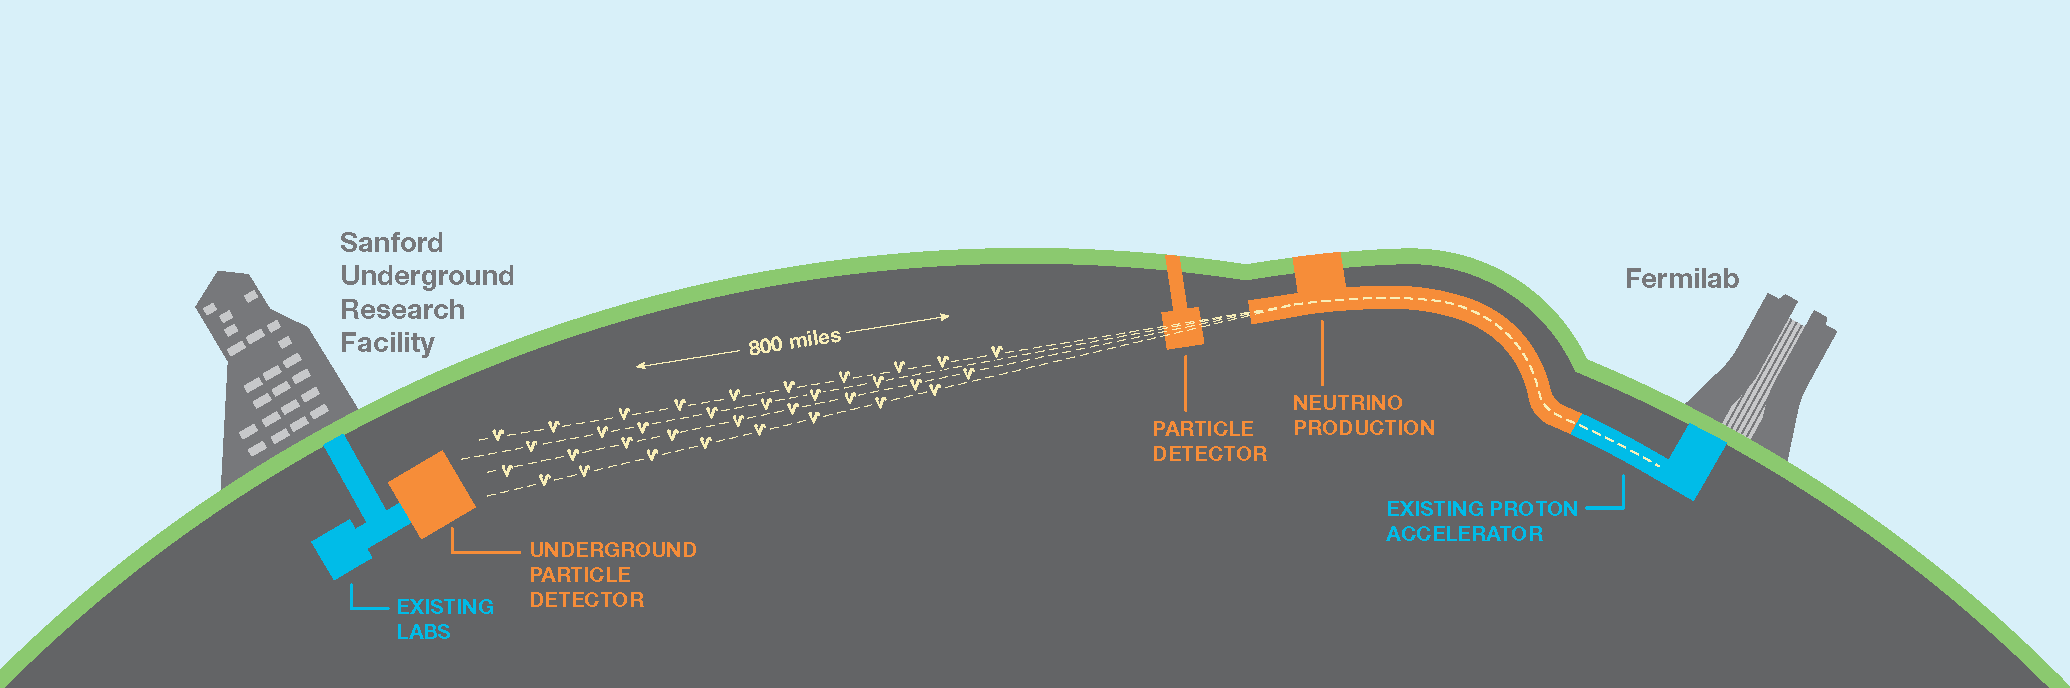
\includegraphics[width=0.95\textwidth, keepaspectratio=true]{figs/LBNF_overallScheme.png} 
\end{figure}

%\subsection{Highlights from LBNF/DUNE Physics Program}
The primary focus of the LBNF will be to measure the neutrino oscillation parameters involved in Formula \ref{eq:P_bigFormula}, especially 
\begin{itemize}
\item determine mass hierarchy (sign of $\Delta{m_{32}}$);
\item measure $\delta$ (to determine whether CP-violation is present in lepton sector); and
\item determine octant of $\theta_{23}$ (now $\theta_{23}$ is indistinguishable from $45^0$, and it is not clear whether the angle is greater, smaller, or equal to $45^0$).
\end{itemize}
To extract the desired quantities, one would build the $P_{\nu_\mu \rightarrow \nu_e}(E_{\nu})$ as a function of neutrino energy and perform a fit of the function, allowing the measured quantities as fit parameters in assumptions of two possible mass hierarchies. The number of electron neutrinos registered at the FD and flux of muon neutrinos measured at the ND integrated over a certain amount of time are related as described by Formula \ref{eq:NnueEspectrum} \cite{ref_Lisa}: \\ 
\begin{center}
\begin{equation}
\label{eq:NnueEspectrum}
N_{\nu_e}(E_{\nu}) = \frac{dN_{\nu_\mu}(E_{\nu})}{dS} \cdot P_{\nu_\mu \rightarrow \nu_e}(E_{\nu}) \cdot \sigma(E_{\nu}) \cdot \epsilon_{\nu_e}, 
\end{equation}
\end{center}
where $N_{\nu_e}(E_{\nu})$ is a number of $\nu_e$, $\frac{dN_{\nu_\mu}(E_{\nu})}{dS}$ is the flux of $\nu_\mu$ in the assumption of no oscillations, $P_{\nu_\mu \rightarrow \nu_e}(E_{\nu})$ is the oscillations probability, $\sigma(E_{\nu})$ is the cross section of $\nu_e$ interaction with a liquid argon nucleon, $\epsilon_{\nu_e}$ is the $\nu_e$ detection efficiency.\\ \\
$N_{\nu_e}(E_{\nu})$ would be measured at the FD, $\frac{dN_{\nu_\mu}(E_{\nu})}{dS}$ would be measured at the ND and then extrapolated to the FD using simulation. Methods used to measure $\sigma(E_{\nu})$ and $\epsilon_{\nu_e}$ in the other neutrino physics experiment (ICARUS) are described in \cite{ref_eff_ICARUS}. $P_{\nu_\mu \rightarrow \nu_e}(E_{\nu})$ is the only unknown term in Formula \ref{eq:NnueEspectrum}, and it would be fit according to Formula \ref{eq:P_bigFormula}.\\ \\
Key advantages of the LBNF/DUNE experiment compared to other long baseline neutrino experiments (Tab. \ref{tab:compareExps}), are a longer baseline which would make the experiment more sensitive to mass hierarchy and CP-violation, higher beam power which would produce more neutrinos and a larger FD mass which would allow to register neutrinos more effectively. \\ \\
Volume 2 of \cite{ref_LBNF_CDR} reports the results of the experiment sensitivity study, calculates expected significances of each of the values to be measured for different values of exposure. Exposure of the experiment is defined as beam power multiplied by the FD mass and by time length of data taking and expressed in $MW \cdot kt \cdot years$ units. For design beam power of 1.07 MW and the FD mass of 40 kt, an exposure of 300 $MW \cdot kt \cdot years$ would correspond to $\sim$7 years of data-taking for reference beam design. For upgraded beam power of 2.4 MW, 300 $MW \cdot kt \cdot years$ would correspond to $\sim$3 years of data taking.\\ \\
Expected exposures necessary to reach certain physics goals for reference beam are summarized in Tab. \ref{tab:exposures_needed}. \\ \\
The idea of LBNF/DUNE limitations can be extracted from Fig. \ref{fig:sensitivity}. The left and the middle plots show expected significances of the MH and the CP determinations as functions of $\delta/\pi$ for certain values of mixing angles. The MH can be determined with almost $5\sigma$ significance for any value of $\delta$ with an exposure of 300 $MW \cdot kt \cdot years$. \\ \\
As for the phase $\delta$, it is shown in Fig. \ref{fig:sensitivity} (middle) that significance of its measurement drops dramatically as $\delta$ approaches 0 or $\pm\pi$ values. The plot shows that for an exposure of 300 $MW \cdot kt \cdot years$, if $|\delta|<0.2\cdot\pi$ or $|\pi-\delta|<0.2\cdot\pi$, then phase $\delta$ can be determined with the significance of less than $3\sigma$. LBNF/DUNE plans on $\sim 20$ years of data taking which would correspond to exposure of $\sim 2000~MW \cdot kt \cdot years$, but even that may not be enough to determine $\delta$ with high enough significance if true value of $\delta$ is close enough to 0 or $\pm\pi$. \\ \\
Fig. \ref{fig:sensitivity} (right) shows that if $|45^0-\theta_{23}|<\sim 2^0$ then the $\theta_{23}$ octant can not be determined with better than $3\sigma$ significance with the same exposure as gives $3\sigma$ significance for 75\% of $\delta$ values. Fig. \ref{fig:sensitivity} shows plots for the NH only but the picture for the IH is similar. More plots, tables and comments about the sensitivity studies are available in \cite{ref_LBNF_CDR}.\\ \\
\begin{table}[h]
  \centering
  \begin{center}
  \caption{ The exposure needed to perform measurements with certain precision expressed in $MW \cdot kt \cdot years$. Estimates provided in the table assume normal mass hierarchy and best fit values of the known parameters. CPV stands for charge-parity violation. }
  \begin{tabular}{|c|c|}
  \hline  
  Physics milestone & Exposure  \\ \hline
   & [$MW \cdot kt \cdot years$]  \\ \hline
%   & (reference beam)  \\ \hline
  $1^0$ $\theta_{23}$ resolution ($\theta_{23}~=~42^0$) & 70 \\ \hline
  CPV at $3\sigma$ $(\delta_{CP}=+\pi/2)$ & 70  \\ \hline
  CPV at $3\sigma$ $(\delta_{CP}=-\pi/2)$ & 160  \\ \hline
  CPV at $5\sigma$ $(\delta_{CP}=+\pi/2)$ & 280  \\ \hline
  MH at $5\sigma$ (at worst) & 400  \\ \hline
  $10^0~\delta_{CP}$ resolution at $\delta_{CP}=0$ & 450  \\ \hline
  CPV at $5\sigma$ $(\delta_{CP}=-\pi/2)$ & 525  \\ \hline
  CPV at $5\sigma$, $50\%$ of $\delta_{CP}$ & 810  \\ \hline
  CPV at $3\sigma$, $75\%$ of $\delta_{CP}$ & 1320  \\ \hline
  \end{tabular}
  \label{tab:exposures_needed}
  \end{center}
\end{table}
\begin{figure}
\caption{LBNF/DUNE sensitivities to the mass hierarchy (left), the CP-violating phase (middle), and the $\theta_{23}$ octant.}
\label{fig:sensitivity}
\centering
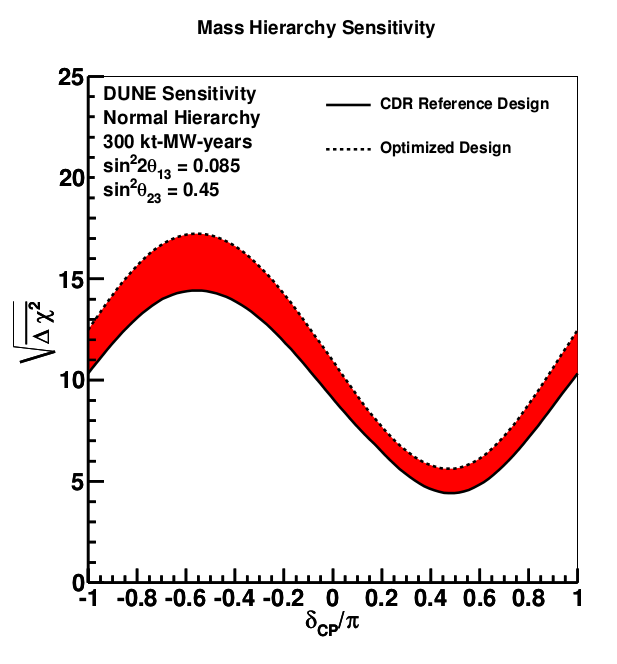
\includegraphics[width=0.30\textwidth, keepaspectratio=true]{figs/sensitivity_MH.png}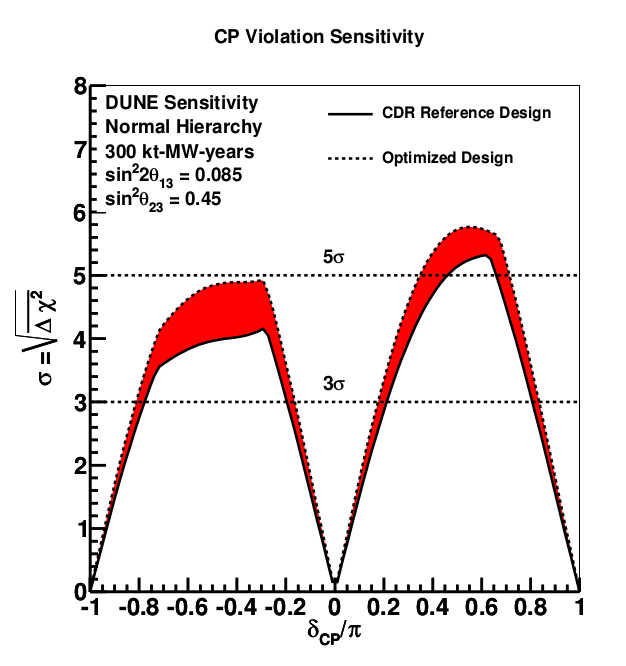
\includegraphics[width=0.31\textwidth, keepaspectratio=true]{figs/sensitivity_CP.png}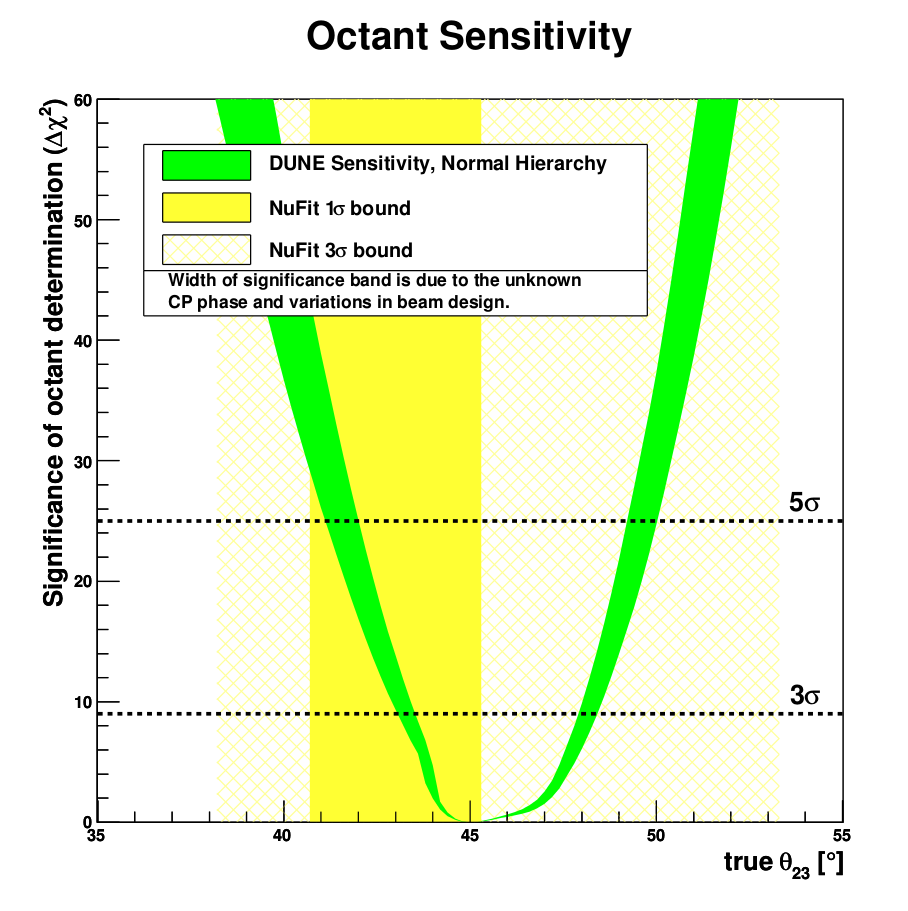
\includegraphics[width=0.32\textwidth, keepaspectratio=true]{figs/sensitivity_theta23.png}
\end{figure}
%%%%%%%%%%%%%%%%%%%%%%%%%%%%%%%%%%%%%%%%
%% if reference beam only
%%%%%%%%%%%%%%%%%%%%%%%%%%%%%%%%%%%%%%%%
%% if also has optimized beam
%\begin{table}[h]
%  \centering
%  \begin{center}
%  \caption{ The exposure needed to perform measurements with certain precision expressed in $MW \cdot kt \cdot years$. Estimates provided in the table assume normal mass hierarchy and best fit values of the known parameters }
%  \begin{tabular}{|c|c|c|}
%  \hline  
%  Physics milestone & Exposure, $MW \cdot kt \cdot years$ & Exposure, $MW \cdot kt \cdot years$ \\ \hline
%   & (reference beam) & (optimized beam) \\ \hline
%  $1^0$ $\theta_{23}$ resolution ($\theta_{23}~=~42^0$) & 70 & 45 \\ \hline
%  CPV at $3\sigma$ $(\delta_{CP}=+\pi/2)$ & 70 & 70 \\ \hline
%  CPV at $3\sigma$ $(\delta_{CP}=-\pi/2)$ & 160 & 100 \\ \hline
%  CPV at $5\sigma$ $(\delta_{CP}=+\pi/2)$ & 280 & 210 \\ \hline
%  MH at $5\sigma$ (at worst) & 400 & 230 \\ \hline
%  $10^0~\delta_{CP}$ resolution at $\delta_{CP}=0$ & 450 & 290 \\ \hline
%  CPV at $5\sigma$ $(\delta_{CP}=-\pi/2)$ & 525 & 320 \\ \hline
%  CPV at $5\sigma$, $50\%$ of $\delta_{CP}$ & 810 & 550 \\ \hline
%  CPV at $3\sigma$, $75\%$ of $\delta_{CP}$ & 1320 & 850  \hline
%  \label{tab:exposures_needed}
%  \end{tabular}
%  \end{center}
%\end{table}

\subsection{Neutrino Beam}

\begin{figure}
\caption{The neutrino beam production at the LBNF. Source of figure: \cite{ref_LBNFweb}}
\label{fig:LBNF_nuBeam}
\centering
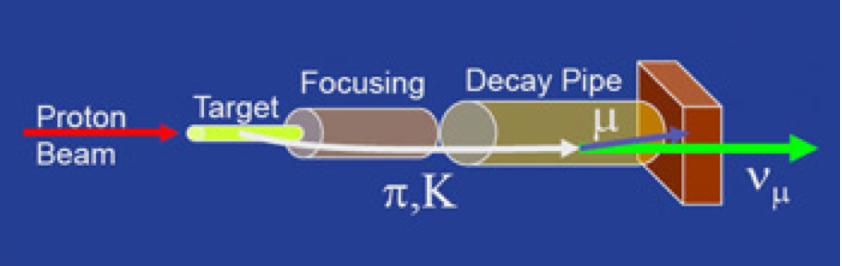
\includegraphics[width=0.45\textwidth, keepaspectratio=true]{figs/LBNF_nuBeam.png}  
\end{figure}


The LBNF neutrino beam will be the highest intensity neutrino beam ever created. The proton accelerator at Fermilab which was already used in other experiments at Fermilab before will produce the beam of protons. Then protons will hit a target and create pions through the reactions $p+p \rightarrow p+n+\pi^+$, $p+p \rightarrow p+\Delta^{++}+\pi^-$, $p+n \rightarrow p+p+\pi^-$, $p+n \rightarrow n+n+\pi^+$, $p+n \rightarrow p+\Delta^{-}+\pi^+$ and kaons through similar reactions which go strongly through gluon. 

%%%%%%%%%%%%%%%%%%%%%%%%%%%%%%%%%%%%%%%%%%%%%%%%%%%%%%
%% Feynman diagrams and descriptions of 
%% how the neutrinos were produced in the target 
%% are probably not necessary 
%%%%%%%%%%%%%%%%%%%%%%%%%%%%%%%%%%%%%%%%%%%%%%%%%%%%%%

%\begin{figure}
%\caption{Examples of the Feynmann diagrams of charged pion and kaon productions in proton-proton scattering.}
%\label{fig:pionAndKaonProductions}
%\centering
%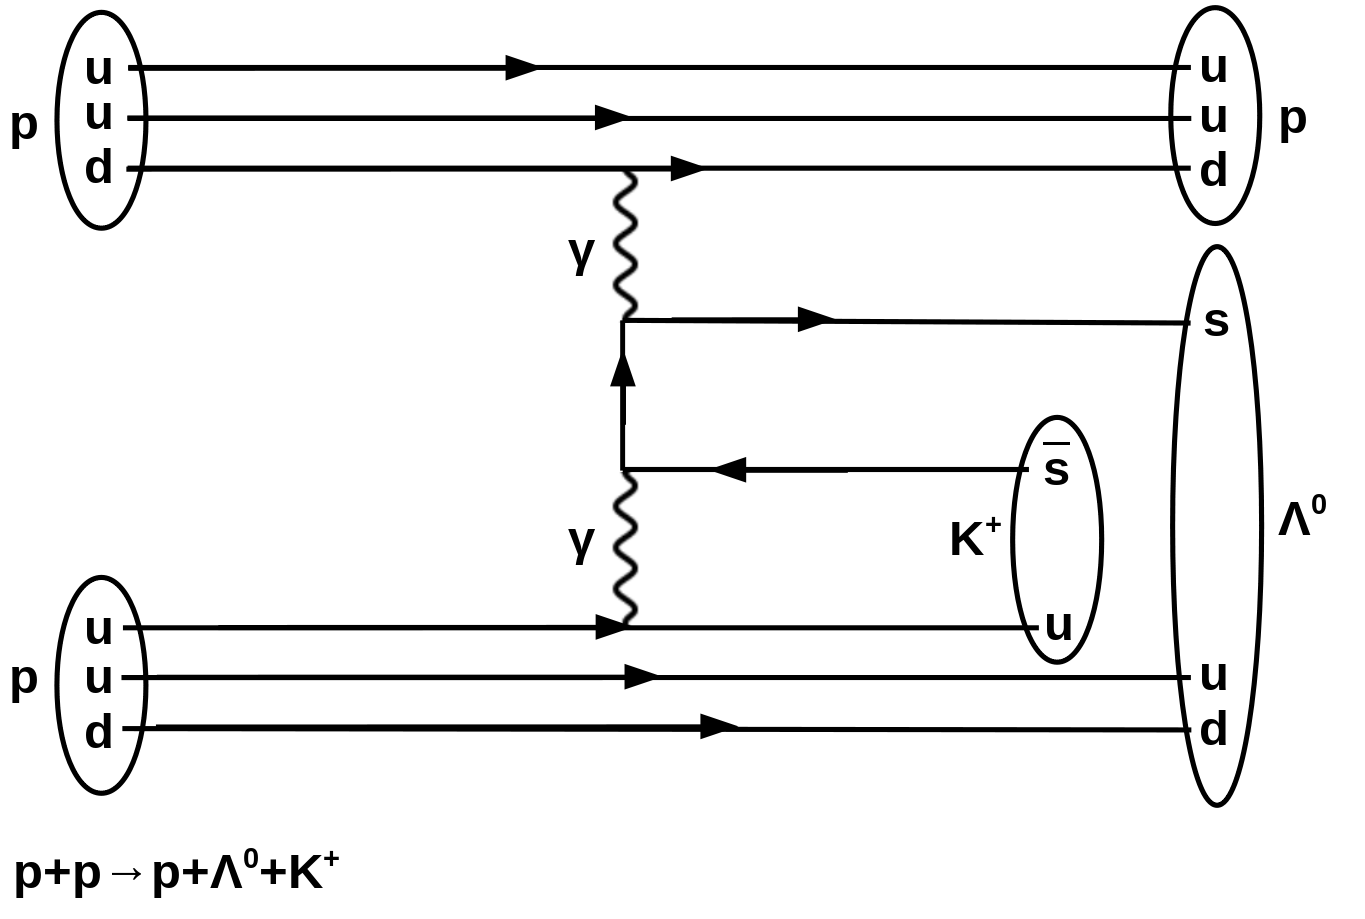
\includegraphics[width=0.48\textwidth, keepaspectratio=true]{figs/ppKaonProduction.png}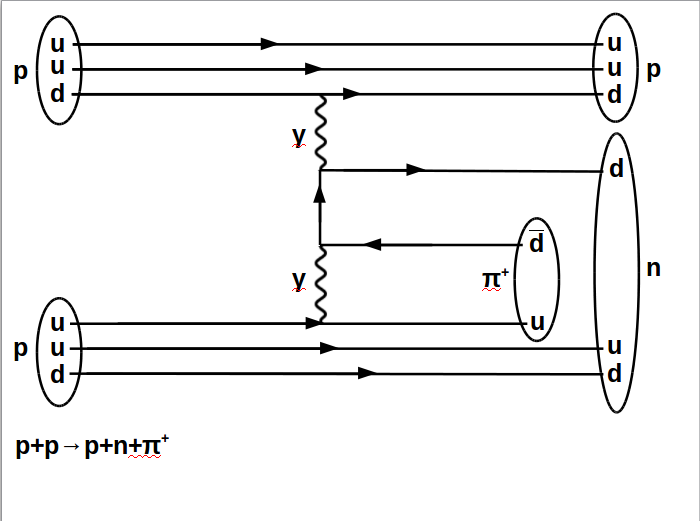
\includegraphics[width=0.48\textwidth, keepaspectratio=true]{figs/ppPionProduction.png}  
%\end{figure}
%In more general words, one quark from the accelerator beam proton scatters on the other quark from the proton or neutron of the target substance as shown at fig. \ref{fig:pionAndKaonProductions}. They exchange gluon which produces quark-antiquark pair. At this moment, the system has seven quarks and one antiquark. The antiquark pairs up with one of the quarks participating in the reaction and the remaining six quarks make two baryons in a way to satisfy color charge neutrality in final particles.  The charged pions have quark compositions $\pi^+ = u\bar{d}$ and $\pi^- = \bar{u}d$ and can be produced with the reactions which only include first generation quarks. The formulas of charged kaons are $K^+ = u\bar{s}$, $K^- = \bar{u}s$. Thus, to produce kaons, the gluon has to produce $s\bar{s}$ pair. 
%\begin{figure}
%\caption{Feynmann diagrams of charged pion and kaon decays to muon and muon antineutrino weakly through W-boson}
%\label{fig:pionAndKaonDecays}
%\centering
%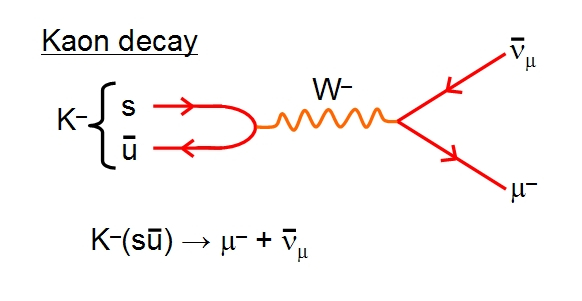
\includegraphics[width=0.45\textwidth, keepaspectratio=true]{figs/kaonDecay.jpg}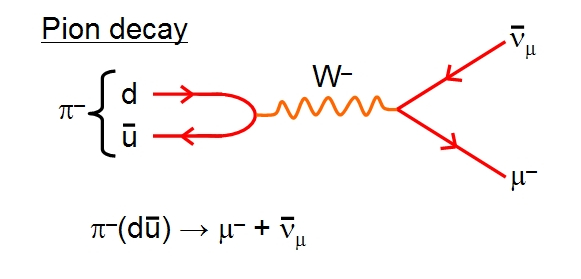
\includegraphics[width=0.45%\textwidth, keepaspectratio=true]{figs/pionDecay.jpg} 
%\end{figure}

After the mesons are created, they go through the focusing system and decay into the decay pipe as $\pi^+ \rightarrow \mu^+\nu_\mu$, $\pi^- \rightarrow \mu^-\bar{\nu_\mu}$, $K^+ \rightarrow \mu^+\nu_\mu$, $K^- \rightarrow \mu^-\bar{\nu_\mu}$ (fig. \ref{fig:pionAndKaonDecays}). The branching ratios of charged pions and kaons to decay into $\mu^+\nu_\mu$($\mu^-\bar{\nu_\mu}$) are $(>99.9)\%$ and $(63.55\pm0.011)\%$ respectively therefore most neutrinos produced into the decay pipe will be muon neutrinos. (While the neutral kaons can also be produced in the target and later decay in pions which could further decay and produce muon neutrinos, the focusing is being done with the certain configuration of the magnetic field and only can affect charged particles. Neutral pions, $\pi^0$s, are very likely to be produced as well but they decay as $\pi^0 \rightarrow \gamma\gamma$ and, therefore, can't contribute to the neutrino production.)\\
After being produced in the reactions described above, the neutrinos will be detected in the near detector at Fermilab. Then the neutrinos will travel 1300 km through the Earth crust and will be detected at SURF in South Dakota.\\  

One of the most important beam requirements is high intensity to produce large enough number of neutrinos to perform intended measurements. Expected beam power of 1.07 MW is expected in the beginning of the experiment with further update to 2.4 MW which is three times larger than the highest beam intensity from other experiments of this kind. Beam production system must be able to work in both muon neutrinos and muon antineutrinos modes. Energies of produced neutrinos must cover the first and the second oscillation nodes which corresponds to energies of 0.5-5 GeV for baseline of 1300 km. Corresponding proton energies are 60-120 GeV.


\subsection{Far Detector}

The main physics goal of the FD would be to measure $N_{\nu_e}(E_{\nu})$  from Formula \ref{eq:NnueEspectrum} but it would also measure $N_{\nu_\mu}(E_{\nu})$ to observe the reduced muon neutrino spectrum. Neutrinos and antineutrinos can produce signal through the CC:

$\nu_f+N \rightarrow f^- + N' +X$, $\bar{\nu_f}+N \rightarrow f^+ + N' +X$,

or through the NC:

$\nu_f+N \rightarrow \nu_f + N +X$, $\bar{\nu_f}+N \rightarrow \bar{\nu_f} + N +X$

where f is e or $\mu$, N is a proton or a neutron, N' is another baryon, and X is other hadrons produced in the reaction.

In case of CC, the produced charged lepton would be fully reconstructed, and also energy of all the final state particles would be summed up to reconstruct the neutrino energy. In case of NC, neutrino would not be detected, such events would be treated as a background.

The FD would be capable to efficiently reconstruct photons, electrons, muons and hadrons. \\

\begin{figure}
\caption{The scheme of the cross section of the LArTPC for far detector of the DUNE and the FD caverns. Sources of figures: \cite{ref_LBNF_CDR}}
\label{fig:farDetector_TPC}
\centering
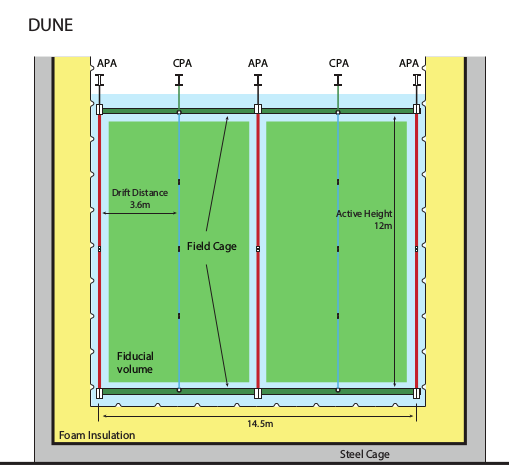
\includegraphics[width=0.5\textwidth, keepaspectratio=true]{figs/farDetector_TPC.png}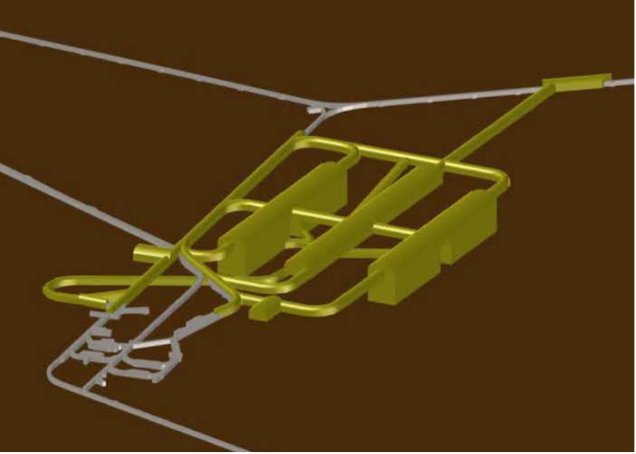
\includegraphics[width=0.5\textwidth, keepaspectratio=true]{figs/farDetector_Caverns.png}
\end{figure}

The LBNF/DUNE FD will be located at SURF in South Dakota. There will be four modules, 10,000 tonnes of liquid argon each, placed into four caverns 1500 m underground. Each module will be 15 m wide, 12 m high and 58 m long, along the beam direction. The caverns will be placed as pairs and there will be the fifth cavern between two pairs - the one with the cryogenic equipment, to provide cooling for liquid argon.\\ 

Key advantages of liquid argon as an FD working volume as described in \cite{ref_aboutLAr} are the ability to act as both a target and a detector, and also to operate as a tracker and a Cherenkov detector at the same time. Liquid argon is denser than water, and therefore such detector would experience more neutrino induced reactions per unit volume than a water detector would. \\

The liquid argon TPC is the main working volume of the detector. The chamber is merged into the liquid argon at a temperature of 89 K. In Figure \ref{fig:farDetector_TPC}, the cathode plane assemblies (CPAs) and the anode plane assemblies (APAs) are shown. The voltages on the APAs and the CPAs are applied in such a way to create a uniform electric field between anode and cathode planes. Charged particle traveling through the electron field ionizes argon atoms. Electrons induced in the ionization process drift to the APAs and produce signal on the readout electronic elements.



\subsection{Near Detector}

The most important physics goal of the ND is to measure the produced muon neutrino flux $\frac{dN_{\nu_\mu}(E_{\nu})}{dS}$ as it would go to Formula \ref{eq:NnueEspectrum}. In the $\nu_\mu$ beam there is also $\nu_e$ contamination present which would be background to $\nu_e$ which would appear as a result of neutrino oscillations at the FD. This background has to be estimated and subtracted. There would be also admixtures of $\bar{\nu_\mu}$ and $\bar{\nu_e}$ in the beam produced. The ND would perform measurement of the overall neutrino and antineutrino flavor composition. 

To measure flavor composition, the ND has to be able to reconstruct muons and electrons, and also to be able to distinguish between the opposite sign leptons. 

\begin{figure}
\caption{Scheme of the DUNE Near Detector (left) and related complex (right).}
\label{fig:nearDetector}
\centering
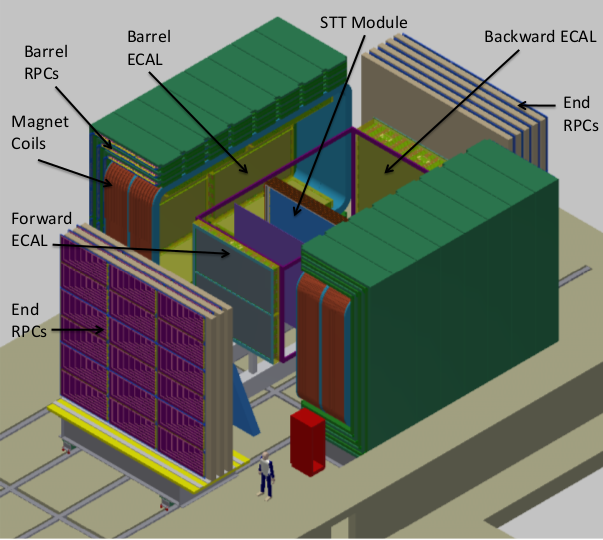
\includegraphics[width=0.63\textwidth, keepaspectratio=true]{figs/nearDetector.png}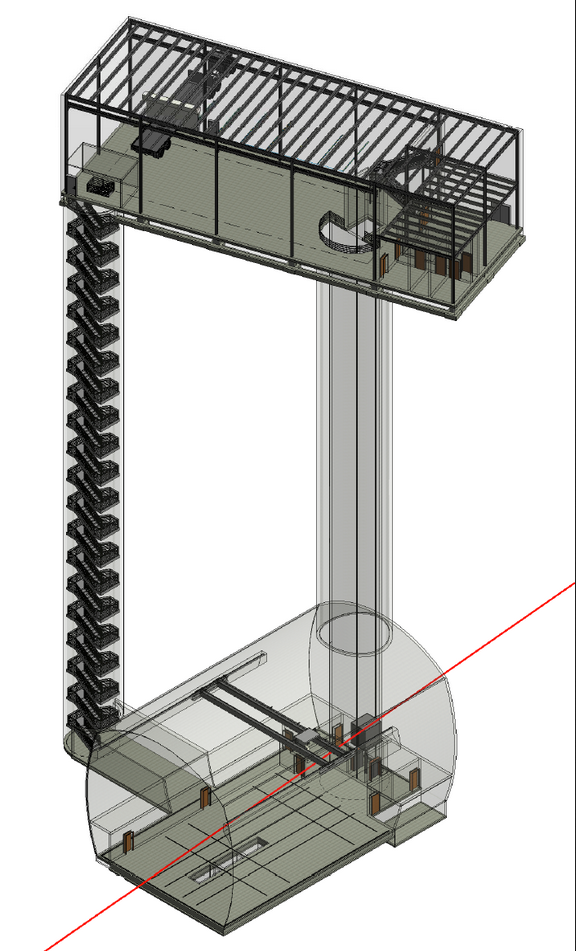
\includegraphics[width=0.35\textwidth, keepaspectratio=true]{figs/nearDetector_project.png}
\end{figure}

The ND would be located few hundred meters downstream the neutrino beam, and the neutrino beam would be much denser at this point than after travelling 1300 km to the FD, that is why the ND doesn't have to be as large as the FD. Also the ND aims on measuring number of neutrinos with much higher precision than the FD to significantly reduce the systematic uncerntainties.\\  

Because of different physics goals, the scheme of the ND (shown at the Fig. \ref{fig:nearDetector}) is also very different from the one of the FD. The detector will consist of central Straw-Tube Tracker (STT) modules, electromagnetic calorimeter (ECAL), magnet coils of 0.4T and muon identification system consisting of Resistive Plate Chamber (RPC) modules. The neutrinos would come from the bottom left corner of the picture, to the End RPCs. The detector will be placed 60 meters underground.





%\subsection{LBNF compared to the other long baseline neutrino oscillation experiments}
Table \ref{tab:compareExps} provides the comparisons of the LBNF/DUNE most important parameters with those of the other long baseline neutrino experiments: K2K, NuMI, CNGS and T2K \cite{ref_LBN_OscExpReview}. The beam power of LBNF/DUNE is planned to be 2.4 MW while the other operating experiments have only beam powers of few hundred Watts. The baseline of LBNF/DUNE is planned to be 1300 km while the baselines of the other experiments vary from 250 km to 735 km only. The Super-Kamiokande FD has a larger mass than the LBNF/DUNE FD is going to have (50 kt vs 40 kt) but the LBNF/DUNE FD will be filled with liquid argon which is a more favorable substance for neutrino detection than water (which the Super-Kamiokande FD is filled with). The only FD which has liquid argon as working volume is ICARUS but its mass is only 0.76 kt. \\ \\
%Therefore, among the experiments discussed, LBNF/DUNE is going to have the longest baseline, the highest beam power and the FD with the highest neutrino detection efficiency. These characteristics will allow LBNF/DUNE to perform more precise measurements than previous and currently existing experiments can do and become sensitive to effects which were not observed before.
\begin{table}[h]
  \centering
  \begin{center}
  \caption{ Comparison of different long baseline neutrino oscillations experiments. Abbreviations and notations used in the table: $E_p$ - proton energy, FGD - Fine-Grained Detector, ChD - Cherenkov Detector, LAr - liquid argon }
  \begin{tabular}{|c|c|c|c|c|c|}
              & KEK (K2K) & NuMI & CNGS & T2K & LBNF/DUNE\\ \hline
     location & Japan  & Illinois - & Switzerland - & Japan & Illinois - \\ 
              &        & Minnesota & Italy &  & South Dakota\\ \hline
     accelerator & KEK PS  & FNAL & CERN's SPS & J-PARC & FNAL\\ \hline
     time of oper. & 1999-2004  & 2005-2012 & 2006-2012 & 2010- & future \\ \hline 
     beam power  &  5 kW  & 300-350 kW  & 300 kW & 750 kW & 2400 kW\\ \hline 
     $E_p$  & 12 GeV & 120 GeV & 400 GeV & 30 GeV & 60-120 GeV\\ \hline 
     baseline  & 250 km & 735 km & 730 km & 295 km & 1300 km\\ \hline 
%                & KEK (K2K)   & NuMI                & CNGS                & T2K         & LBNF (DUNE)\\ \hline
     near        & (water ChD) & MINOS               & (muon               & ND280       & DUNE (FGD)\\  
     detector(s) & (FGD)       & (track. and scint.) & detector)           & INGRID      & \\ \hline 
     ND mass     & 1 kt (ChD)  & 0.98 kt             &                     &             & \\ \hline 
     far         & SuperK      & MINOS               & ICARUS (LAr)        & SuperK      & DUNE (LAr)\\  
     detector(s) & (water ChD) & track. and scint.   & OPERA (FGD)        & (water ChD) & \\ \hline 
     FD mass     & 50 kt       & 5.4 kt              & 0.76 kt (ICARUS)   & 50 kt       & 40 kt\\ 
                 &             &                     & 1.25 kt (OPERA)    &             & \\ \hline 
 \end{tabular}
  \label{tab:compareExps}
  \end{center}
\end{table}


% Summary

LBNF/DUNE is future long baseline neutrino oscillations experiment which will be hosted by two large physics laboratories in USA: Fermilab in Illinois and SURF in South Dakota. LBNF/DUNE's baseline of 1300 km, expected beam power of 2 MW, and 40 kt of liquid argon FD makes LBNF/DUNE the most ambitious neutrino oscillations facility ever created. In addition to precision measurements of such neutrino mixing parameters as $\theta_{12}$, $\theta_{23}$, $\theta_{13}$, $|\Delta{m_{12}}^2|$, $|\Delta{m_{32}}^2|$, it is expected to have enough sensitivity to determine the neutrino mass hierarchy and the CP-violation phase $\delta$ which were never determined before.\\

\clearpage
\section{Conclusions}
Neutrino oscillations were first observed in the 1960s and confirmed in 1998. Neutrinos were believed to be massless for a long time, but the oscillations assume neutrinos to be massive. This phenomenon made the scientific community rethink the theory of weak interactions. While several possible theoretical frameworks to incorporate neutrino masses into the Standard Model have been suggested, it is not clear which hypothesis is true. Precision measurement of neutrino oscillation parameters may bring insight into the understanding of matter-antimatter asymmetry in the Universe and general picture of the generations of the fundamental Standard Model particles. \\ \\
Neutrino oscillations can be described with four parameters of the neutrino mixing matrix (three angles $\theta_{12}$, $\theta_{23}$, $\theta_{13}$ and complex CP-violating phase $\delta$) and the two mass differences (${\Delta}m_{21}$ and ${\Delta}m_{32}$).\\ \\
Neutrino oscillations can be studied with solar, atmospheric, reactor, or accelerator neutrino experiments. The key idea of any neutrino oscillation experiment is to observe and quantitatively describe disappearance of neutrinos/antineutrinos which were produced and/or appearance of neutrinos/antineutrinos which were not produced. Then probability of neutrinos to oscillate is built and fitted with the assumptions of a certain model, and the neutrino oscillation parameters are extracted.\\ \\
Significant progress was made in recent years in neutrino oscillation physics with all four types of experiments. Three angles $\theta_{12}$, $\theta_{23}$, $\theta_{13}$ have been measured with several degrees precision, absolute values of ${\Delta}m_{21}$ and ${\Delta}m_{32}$ were measured too, and it is known that $m_2 > m_1$. However, all previous experiments were not sensitive enough to determine the sign of ${\Delta}m_{32}$ and the phase $\delta$.\\ \\
That is why the new LBNF/DUNE experiment was proposed. It will be an accelerator long baseline neutrino oscillations experiment. The highest ever neutrino beam power, the longest baseline and the most effective far detector would make LBNF/DUNE the most ambitious neutrino oscillations experiment in the world and sensitive to effects which were not observed by any other experiment to date. LBNF/DUNE is expected to determine the sign of ${\Delta}m_{32}$ with high significance, phase $\delta$ in broad range of values, and provide the most precise test of the three-neutrino oscillations theory.\\ \\

\clearpage
%\section{References}
\begin{thebibliography}{1}
   % Intro
   \bibitem{ref_fig_StandardModel} website: http://www.isgtw.org/spotlight/go-particle-quest-first-cern-hackfest
   \bibitem{ref_Griffiths} David Griffiths "Introduction to Elementary Particles", Wiley-VCH; 2nd edition (October 13, 2008)
   \bibitem{ref_PDG} K.A. Olive et al. (Particle Data Group), Chin. Phys. C, 38, 090001 (2014) 
   % Theory
   \bibitem{ref_theory_Osc} H. Nunokawa, S. J. Parke, and J. W. Valle, “CP Violation and Neutrino Oscillations,”
Prog.Part.Nucl.Phys., vol. 60, pp. 338–402, 2008.
   \bibitem{ref_LBNF_CDR} LBNF CDR draft: https://web.fnal.gov/project/LBNF/SitePages/LBNF\%20Reports\%20and\%20Papers.aspx
   % History/Status
   \bibitem{ref_presentation_MH} presentation by Jarah Evslin in INFN Sezione di Torino seminar: http://www.astroparticle.to.infn.it/seminari/files/140620-Evslin.pdf
   %LBNF/DUNE Project
   \bibitem{ref_LBNFweb} LBNF website: http://lbnf.fnal.gov/
   \bibitem{ref_Lisa} personal e-mail from Prof. Lisa Whitehead
   \bibitem{ref_eff_ICARUS} M. Bhattacharya et al. Neutrino absorption efficiency of an $^{40}Ar$ detector from the $\beta$ decay of $^{40}Ti$, Phys. Rev. C 58, 3677 – Published 1 December 1998
   \bibitem{ref_aboutLAr} website Fermilab today: http://www.fnal.gov/pub/today/archive/archive\_2014/today14-10-09.html
   \bibitem{ref_LBN_OscExpReview} G. J. Feldman, J. Hartnell, T. Kobayashi, A Review of Long-baseline Neutrino Oscillation Experiments, Advances in High Energy Physics 2013 (2013), 475749
\end{thebibliography}

\clearpage



\end{document}
